% Provenance (never printed): NSI premiere project closing the year: "Architectures materielles: modele de von Neumann,
% langage assembleur" turned into a programming project (assembler + simulator). See sources/book2/BRIEFS.md.
\chapter{Project: An Assembler and Simulator for the Toy Machine}\label{ch:g11:project-toy-machine}

Every program of the toy machine in this book has so far been assembled and run by a tool that came with the series.
This project rebuilds both halves of that tool in Python: the \omterm{def:g11:von-neumann-machine:assembly}{assembler}, which turns the text of a program into
bytes, and the \omterm{def:g11:project-toy-machine:simulator}{simulator}, which runs the bytes one instruction at a time. When the project is finished, the two
tools must agree with the series' own, byte for byte and step for step, on every program of chapter
\ref{ch:g11:von-neumann-machine}.

\begin{recall}
The toy machine: $256$ cells of one byte, four registers, \code{PC} and \code{SP}, the flags Z, N and C, $28$
instructions of two bytes each (chapter \ref{ch:g11:von-neumann-machine}). Numbers modulo $256$ and \omterm{def:g10:machine-integers:twos-complement}{two's complement}
(chapter \ref{ch:g10:machine-integers}). Modules and their interfaces, and tests that check an \omterm{def:g11:modules-and-interfaces:interface}{implementation} against
another (chapter \ref{ch:g11:modules-and-interfaces}).
\end{recall}

\section{The specification}\label{sec:g11:project-toy-machine:spec}

Write, in Python, a \omterm{def:g11:project-toy-machine:two-pass}{two-pass assembler} for the toy machine's \omterm{def:g11:von-neumann-machine:assembly}{assembly language}, with labels, comments, the four ways
of writing a number and \code{DATA}; and a \omterm{def:g11:project-toy-machine:simulator}{simulator} of its fetch--execute cycle with the $28$ instructions, the flags,
the stack, \code{IN} and \code{OUT}, a limit on the number of steps and a trace. Check both against the series'
package \code{toymachine} on every program of chapter \ref{ch:g11:von-neumann-machine}: same bytes, same outputs, same
final state, same trace.

The shared package is used only to compare: the chapter's code adds its folder to \code{sys.path} and imports it,
never changes it. The work goes in five milestones, each one runnable before the next starts.

\begin{omfigure}
\begin{tikzpicture}[box/.style={draw, rounded corners=2pt, minimum height=8mm, align=center, font=\footnotesize},
    ->, >=stealth]
  \node[box, fill=black!5] (src) at (0,0) {source text\\ \code{.toy}};
  \node[box, fill=omDef!10] (p1) at (3.1,0) {pass 1:\\ count bytes};
  \node[box, fill=omMeth!12] (sym) at (3.1,-1.8) {symbol table\\ \texttt{\{\textquotesingle{}loop\textquotesingle{}: 6, \dots\}}};
  \node[box, fill=omDef!10] (p2) at (6.4,0) {pass 2:\\ encode};
  \node[box, fill=black!5] (mem) at (9.6,0) {$256$ bytes\\ of memory};
  \node[box, fill=omThm!10] (sim) at (9.6,-1.8) {simulator:\\ fetch, decode, execute};
  \draw (src) -- node[above, font=\scriptsize] {rows} (p1);
  \draw (p1) -- (sym);
  \draw (sym) -| (p2);
  \draw (p1) -- node[above, font=\scriptsize] {rows} (p2);
  \draw (p2) -- (mem);
  \draw (mem) -- (sim);
\end{tikzpicture}

{\small The two passes. The first only counts bytes, to learn the address of every label; the second encodes each
line, replacing labels by their addresses. The \omterm{def:g11:project-toy-machine:simulator}{simulator} receives the bytes, not the text.}
\end{omfigure}

\section{Milestone 1: reading the lines}\label{sec:g11:project-toy-machine:m1}

A line of assembly has up to three parts: a label ending in a colon, a mnemonic, and operands separated by commas;
a semicolon starts a comment, unless it stands between quotes as a character. The first module turns each line into
a tuple \code{(line number, label, mnemonic, operands)}. Its function \code{parse_number(tok, line)}, not shown, turns
a number written in decimal, hexadecimal, binary or as a character into a byte, and refuses anything that does not
fit; writing it is exercise \ref{exo:g11:project-toy-machine:5}.

\omcode{code/grade-11/10-project-toy-machine/listings/tokens.py}{19}{52}{Milestone 1: names, comments, and one line cut
into its parts.}\label{lst:g11:project-toy-machine:tokens}

\omoutput{code/grade-11/10-project-toy-machine/outputs/run_m1.txt}{The rows of a small program, then seven numbers;
each error names its line.}\label{out:g11:project-toy-machine:m1}

\section{Milestone 2: two passes}\label{sec:g11:project-toy-machine:m2}

\begin{definition}[Two-pass assembler, symbol table]\label{def:g11:project-toy-machine:two-pass}
A \emph{two-pass assembler}\index{two-pass assembler} reads the program twice. The first pass computes the address of
every line and records each label with its address in the \emph{symbol table}\index{symbol table}; the second pass
encodes every line, looking up in the table the labels used as operands.
\end{definition}

Two passes are needed because a label may be used before the line that defines it: \code{JZ done} comes before
\code{done:}. The first pass needs only sizes: two bytes per instruction, one per number of a \code{DATA} line.

\omcode{code/grade-11/10-project-toy-machine/listings/assembler_m2.py}{1}{40}{Milestone 2: the table of operations,
and the first pass.}\label{lst:g11:project-toy-machine:pass1}

\omcode{code/grade-11/10-project-toy-machine/listings/assembler_m2.py}{42}{79}{Milestone 2: encoding one line as
$4 \times \text{opcode} + r$, then the operand.}\label{lst:g11:project-toy-machine:encode}

\omcode{code/grade-11/10-project-toy-machine/listings/assembler_m2.py}{81}{98}{Milestone 2: the second pass, and the
whole \omterm{def:g11:von-neumann-machine:assembly}{assembler}.}\label{lst:g11:project-toy-machine:pass2}

\omoutput{code/grade-11/10-project-toy-machine/outputs/run_m2.txt}{\code{sum_array.toy}: the \omterm{def:g11:project-toy-machine:two-pass}{symbol table}, then the
bytes of every line.}\label{out:g11:project-toy-machine:m2}

\begin{omfigure}
\begin{tikzpicture}[x=0.5cm, y=1cm, font=\scriptsize]
  \foreach \a/\t in {0/LOADI, 2/LOADI, 4/LOAD, 6/LOADR, 8/ADD, 10/ADDI, 12/ADDI, 14/JNZ, 16/OUT, 18/HALT} {
    \draw[fill=omDef!10] (\a,0) rectangle (\a+2,0.8);
    \node[above, font=\tiny] at (\a,0.8) {\a};
    \node[font=\tiny\ttfamily] at (\a+1,0.4) {\t};
  }
  \foreach \v [count=\i from 20] in {6,12,7,30,1,25,9} {
    \ifnum\i=20 \def\fillc{omMeth!20}\else\def\fillc{omThm!12}\fi
    \draw[fill=\fillc] (\i,0) rectangle (\i+1,0.8);
    \node at (\i+0.5,0.4) {\v};
  }
  \node[above, font=\tiny] at (20,0.8) {20};
  \node[above, font=\tiny] at (21,0.8) {21};
  \node[above, font=\tiny] at (27,0.8) {27};
  \draw[omThm, ->] (6,-0.7) node[below] {loop $\to 6$} -- (6,-0.05);
  \draw[omThm, ->] (17.5,-0.7) node[below] {length $\to 20$} -- (20,-0.05);
  \draw[omThm, ->] (23.5,-0.7) node[below] {array $\to 21$} -- (21,-0.05);
\end{tikzpicture}

{\small The memory after assembling \code{sum_array.toy}: ten instructions of two bytes, then seven bytes of
\code{DATA}. Each label of the \omterm{def:g11:project-toy-machine:two-pass}{symbol table} points at an address; the rest of memory, from $27$ to $255$, is free,
and the stack grows down from the top.}
\end{omfigure}

The output is compared with the shared \omterm{def:g11:von-neumann-machine:assembly}{assembler} in milestone~5: for every program, the $256$ bytes are the same.

\section{Milestone 3: the core of the simulator}\label{sec:g11:project-toy-machine:m3}

\begin{definition}[Simulator]\label{def:g11:project-toy-machine:simulator}
A \emph{simulator}\index{simulator} is a program that imitates a machine: it keeps the machine's state in its own
variables and changes it, step by step, as the machine would.
\end{definition}

The state is a dictionary: memory, registers, \code{PC}, \code{SP}, flags, inputs and outputs. Each instruction is a
small function of the machine, the register field and the operand byte; a dictionary maps each operation code to its
function. This milestone gives the cycle and seven instructions only, enough for a first program.

\begin{omfigure}
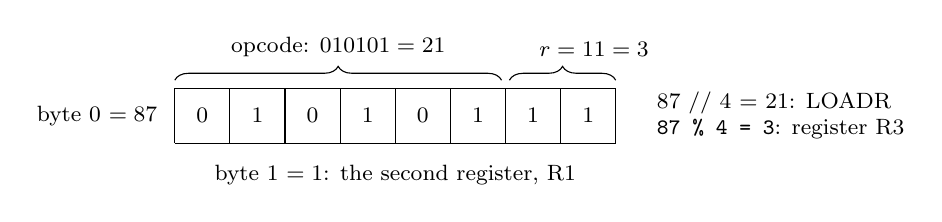
\begin{tikzpicture}[font=\footnotesize]
  \draw[step=0.7] (0,0) grid (5.6,0.7);
  \foreach \b [count=\i from 0] in {0,1,0,1,0,1,1,1} \node at (0.35+0.7*\i,0.35) {\b};
  \draw[decorate, decoration={brace, amplitude=5pt}] (0,0.8) -- node[above=5pt] {opcode: $010101 = 21$} (4.15,0.8);
  \draw[decorate, decoration={brace, amplitude=5pt}] (4.25,0.8) -- node[above=5pt, xshift=4mm] {$r = 11 = 3$}
    (5.6,0.8);
  \node[left] at (-0.1,0.35) {byte 0 $= 87$};
  \node[right, align=left] at (6,0.35) {\code{87 // 4 = 21}: \code{LOADR}\\ \texttt{87 \% 4 = 3}: register R3};
  \node[below, align=center] at (2.8,-0.15) {byte 1 $= 1$: the second register, R1};
\end{tikzpicture}

{\small Decoding the instruction at address $6$ of \code{sum_array.toy}. The top six bits of the first byte are the
operation code, the bottom two the register: \code{LOADR R3, R1}.}
\end{omfigure}

\omcode{code/grade-11/10-project-toy-machine/listings/simulator_m3.py}{1}{40}{Milestone 3: the state, and seven
instructions.}\label{lst:g11:project-toy-machine:m3-ops}

\omcode{code/grade-11/10-project-toy-machine/listings/simulator_m3.py}{43}{65}{Milestone 3: one step of the cycle, and
running with a limit.}\label{lst:g11:project-toy-machine:m3-cycle}

\omoutput{code/grade-11/10-project-toy-machine/outputs/run_m3.txt}{A copy through memory, then a loop with no
\code{HALT}, stopped by the limit.}\label{out:g11:project-toy-machine:m3}

\begin{omfigure}
\begin{tikzpicture}[st/.style={draw, rounded corners=3pt, minimum width=20mm, minimum height=8mm,
    font=\footnotesize, align=center}, ->, >=stealth, font=\scriptsize]
  \node[st, fill=omDef!10] (f) at (0,0) {fetch\\ $b_0, b_1$};
  \node[st, fill=omDef!10] (d) at (3.4,0) {decode\\ opcode, $r$};
  \node[st, fill=omDef!10] (e) at (6.8,0) {execute};
  \node[st, fill=omMeth!15] (h) at (6.8,-1.9) {halted};
  \node[st, fill=omThm!12] (x) at (0,-1.9) {error};
  \draw (f) -- node[above] {PC += 2} (d);
  \draw (d) -- (e);
  \draw (e) -- node[right] {HALT} (h);
  \draw (e.north) to[bend right=30] node[above] {otherwise, if steps $<$ limit} (f.north);
  \draw (f) -- node[left, align=right] {PC past 254,\\ steps $=$ limit} (x);
  \draw (d) -- node[below, sloped] {unknown opcode} (x);
\end{tikzpicture}

{\small The \omterm{def:g11:project-toy-machine:simulator}{simulator}'s loop. Each step fetches two bytes, adds $2$ to \code{PC}, decodes and executes; it stops at
\code{HALT}, or with an error that names the cause.}
\end{omfigure}

\section{Milestone 4: flags, jumps and the stack}\label{sec:g11:project-toy-machine:m4}

The fourth module imports the third and extends its table: the twenty-one other instructions. Arithmetic sets the
flags in one place, \code{set_flags}; the jumps read them.

\omcode{code/grade-11/10-project-toy-machine/listings/simulator_m4.py}{1}{32}{Milestone 4: flags, and the arithmetic
that sets them.}\label{lst:g11:project-toy-machine:m4-arith}

\omcode{code/grade-11/10-project-toy-machine/listings/simulator_m4.py}{35}{63}{Milestone 4: \omterm{def:g11:von-neumann-machine:jump}{conditional jumps}, and
\code{IN}.}\label{lst:g11:project-toy-machine:m4-jumps}

\omcode{code/grade-11/10-project-toy-machine/listings/simulator_m4.py}{65}{99}{Milestone 4: memory through a register,
the stack, \omterm{def:g11:von-neumann-machine:subroutine}{subroutines}.}\label{lst:g11:project-toy-machine:m4-stack}

\code{AND}, \code{OR} and \code{XOR} are made by one function \code{logic}, and the shifts follow the flags'
specification; those lines are not shown (\code{NOT} and \code{SHR} are exercise
\ref{exo:g11:project-toy-machine:7}). The module ends with the full table and a \code{run} that uses it.

\omcode{code/grade-11/10-project-toy-machine/listings/simulator_m4.py}{119}{128}{Milestone 4: the table of the $28$
instructions.}\label{lst:g11:project-toy-machine:m4-table}

\omoutput{code/grade-11/10-project-toy-machine/outputs/run_m4.txt}{Six programs of chapter
\ref{ch:g11:von-neumann-machine}; after the \omterm{def:g11:von-neumann-machine:subroutine}{subroutine} of \code{call_square}, \code{SP} is back at $0$.}%
\label{out:g11:project-toy-machine:m4}

\section{Milestone 5: tests and a trace}\label{sec:g11:project-toy-machine:m5}

The trace prints, before each step, the instruction about to run and the state, in the shared tool's format; a
disassembler turns two bytes back into text.

\omcode{code/grade-11/10-project-toy-machine/listings/trace_m5.py}{1}{28}{Milestone 5: two bytes back to text, and one
row of the trace.}\label{lst:g11:project-toy-machine:trace}

\omcode{code/grade-11/10-project-toy-machine/listings/run_m5.py}{1}{22}{Our trace of \code{max2.toy}, compared with the
shared tool's, character for character.}\label{lst:g11:project-toy-machine:m5}

\omoutput{code/grade-11/10-project-toy-machine/outputs/run_m5.txt}{The two traces are the same
text.}\label{out:g11:project-toy-machine:m5}

Then every program of chapter \ref{ch:g11:von-neumann-machine}, with its inputs, goes through both \omterm{def:g11:modules-and-interfaces:interface}{implementations}.

\omcode{code/grade-11/10-project-toy-machine/listings/compare_shared.py}{1}{25}{Ours against the shared package, on
every program.}\label{lst:g11:project-toy-machine:compare}

\omoutput{code/grade-11/10-project-toy-machine/outputs/compare_shared.txt}{Eight programs: same bytes, same outputs,
same memory, registers, flags and counts at the end.}\label{out:g11:project-toy-machine:compare}

Finally, a test file keeps the checks for every later change, including the errors: each faulty program must be
refused by both \omterm{def:g11:von-neumann-machine:assembly}{assemblers}, and every addition of two bytes must set the same flags in both \omterm{def:g11:project-toy-machine:simulator}{simulators}.

\omcode{code/grade-11/10-project-toy-machine/listings/ours_tests.py}{1}{17}{The tests, first part: the shared package,
the programs, and six faulty ones.}\label{lst:g11:project-toy-machine:tests-data}

\omcode{code/grade-11/10-project-toy-machine/listings/ours_tests.py}{20}{51}{The tests, second part: bytes, errors,
flags and the step limit.}\label{lst:g11:project-toy-machine:tests}

\omoutput{code/grade-11/10-project-toy-machine/outputs/run_ours_tests.txt}{All four
pass.}\label{out:g11:project-toy-machine:tests}

\begin{remark}
The tests of the chapter's own folder go further: the trace of every program, and $300$ random memories run for $40$
steps by both \omterm{def:g11:project-toy-machine:simulator}{simulators}, compared after every step.
\end{remark}

\section{Exercises}\label{sec:g11:project-toy-machine:exercises}

\begin{exercise}[$\star$]\label{exo:g11:project-toy-machine:1}
Give the \omterm{def:g11:project-toy-machine:two-pass}{symbol table} of \code{multiply.toy} (chapter \ref{ch:g11:von-neumann-machine}): six instructions come before
\code{loop:}, and three more before \code{done:}.
\end{exercise}

\begin{exercise}[$\star$]\label{exo:g11:project-toy-machine:2}
How many bytes does the line \code{DATA 1, 2, 3} place in memory, and which?
\end{exercise}

\begin{exercise}[$\star$]\label{exo:g11:project-toy-machine:3}
What does the \omterm{def:g11:von-neumann-machine:assembly}{assembler} of milestone~2 report for the one-line program \code{JMP finish}?
\end{exercise}

\begin{exercise}[$\star$]\label{exo:g11:project-toy-machine:4}
The first byte of an instruction is \code{0x51}. Which operation, and which register?
\end{exercise}

\begin{exercise}[$\star$]\label{exo:g11:project-toy-machine:5}
Write \code{parse_number(tok)} for the four notations, \code{42}, \code{0x2A}, \code{0b101010} and \texttt{\textquotesingle{}*\textquotesingle{}}, with
negative numbers from $-128$ stored in \omterm{def:g10:machine-integers:twos-complement}{two's complement}, and an error for anything outside $-128$ to $255$.
\end{exercise}

\begin{exercise}[$\star\star$]\label{exo:g11:project-toy-machine:6}
A student writes a one-pass \omterm{def:g11:von-neumann-machine:assembly}{assembler}, which encodes each line as soon as it reads it. It works on
\code{count_down.toy} and fails on \code{multiply.toy}. Why? Name two ways to repair it.
\end{exercise}

\begin{exercise}[$\star\star$]\label{exo:g11:project-toy-machine:7}
Write \code{not_(m, r, b)} and \code{shr(m, r, b)} for the \omterm{def:g11:project-toy-machine:simulator}{simulator}, with the flags of the specification, using
neither \texttt{\textasciitilde} nor \code{>>}.
\end{exercise}

\begin{exercise}[$\star\star$]\label{exo:g11:project-toy-machine:8}
A student sets the carry of \code{SUB} and \code{CMP} with \code{a >= b} instead of \code{a < b}. Which programs of
\code{compare_shared.py} now print a wrong result, and what do they print?
\end{exercise}

\begin{exercise}[$\star\star$]\label{exo:g11:project-toy-machine:9}
How many cells of memory are left for the stack while \code{sum_array.toy} runs? Could a deep chain of calls
overwrite the program?
\end{exercise}

\begin{exercise}[$\star\star$]\label{exo:g11:project-toy-machine:10}
Write \code{dump(m)}, which returns the text printed by the shared tool's \code{run --dump}: one line with the
registers, \code{PC}, \code{SP} and the flags, then the non-zero cells, eight per line, as \code{M[a]=v}.
\end{exercise}

\begin{exercise}[$\star\star$]\label{exo:g11:project-toy-machine:11}
Write the trace rows of this program: \code{LOADI R0, 250}, \code{ADDI R0, 10}, \code{JC big}, \code{HALT},
\code{big: OUT R0}, \code{HALT}.
\end{exercise}

\begin{exercise}[$\star\star\star$]\label{exo:g11:project-toy-machine:12}
Add to the \omterm{def:g11:von-neumann-machine:assembly}{assembler} a pseudo-instruction \code{INC r}, which the \omterm{def:g11:von-neumann-machine:assembly}{assembler} expands into \code{ADDI r, 1}. Where in the
two passes does the expansion go, and why does the \omterm{def:g11:project-toy-machine:two-pass}{symbol table} stay right?
\end{exercise}

\begin{exercise}[$\star\star\star$]\label{exo:g11:project-toy-machine:13}
Prove that every pair of bytes whose first byte is below $112$ disassembles into exactly one instruction, and that
assembling that text gives back the same two bytes when the unused fields are $0$.
\end{exercise}

\begin{exercise}[$\star\star\star$]\label{exo:g11:project-toy-machine:14}
Write \code{disassemble_program(memory, end)}, which disassembles the instructions before address \code{end} and
shows the non-zero bytes after it as one \code{DATA} line. Try it on \code{sum_array.toy} with \code{end = 20}.
\end{exercise}

\begin{exercise}[$\star\star\star$]\label{exo:g11:project-toy-machine:15}
How many different instructions does the encoding allow, counting each choice of register, number or address, with
the unused fields at $0$?
\end{exercise}
